\documentclass[tikz, border=1mm,12pt]{standalone}
\usepackage{ebgaramond-maths}
\begin{document}
	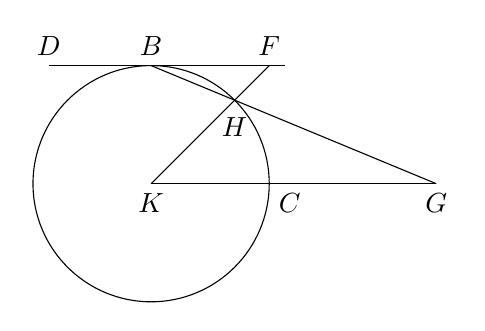
\begin{tikzpicture}
		\draw (0,0) circle (1.5);
		\draw (-1.3,1.5) node[above]{$D$} -- (1.7,1.5);
		\draw (0,0) node[below]{$K$} -- ({(3+3*sqrt(2))/2},0) node[below]{$G$};
		\draw (0,0) -- (1.5,1.5) node[above]{$F$};
		\draw (0,1.5) node[above]{$B$} -- ({(3+3*sqrt(2))/2},0);
		\node[below right] at (1.5,0) {$C$};
		\node[below, outer sep=3] at ({sqrt(1.125)},{sqrt(1.125)}) {$H$};
	\end{tikzpicture}
\end{document}